\section{Introduction}
% what is ``Space subdivision''
Subdivision is the process of partitioning a space $\mathcal{S}$, according to a provided set of level-curves $\mathcal{C}$ in that space, into a set of faces $\mathcal{F}$.
%% \footnote{for simplicity, level-curves will be refered to as curves in the rest of the document.} 

\[ \mathit{subdivision}(\mathcal{C}): \mathcal{S} \xrightarrow[]{decompose} \mathcal{F}\left(\mathcal{C}\right) \]

Figure~\ref{fig:intro_curvesPartitioning1} shows an example of a planar subdivision (where $\mathcal{S}$ is two dimensional), according to a set of curves containing six straight lines.
% what is it useful for? some application?
The process of subdivision provides an abstraction of the space.
Such an abstraction potentially facilitates some geometric processes required on that space.

\begin{figure}%[!ht]
  \centering
  \begin{subfigure}{.4\textwidth}
    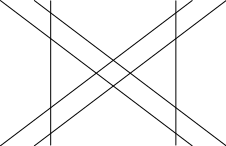
\includegraphics[width=\textwidth]{figures/intro_curves1.png}
    \caption{curves} \label{subfig:intro_curves1}
  \end{subfigure}%
  \quad \quad \quad%
  \begin{subfigure}{.4\textwidth}
    \includegraphics[width=\textwidth]{figures/intro_partitioning1.png}
    \caption{partitionaing} \label{subfig:intro_partitioning1}
  \end{subfigure}%
  \caption[xxx]
          {A planar subdivision, over a set of six straight lines.
          Figure~\ref{subfig:intro_curves1} shows the set of curves, and the ``faces'' resulting from partitioning are color coded in figure~\ref{subfig:intro_partitioning1}.}
  \label{fig:intro_curvesPartitioning1}
\end{figure}

%%%%%%%%%%%%%%%%%%%%%%%%%%%%%%%%%%%%%%%%%%%%%%%%%%%%%%%%%%%%%%%%%%%%%%%%%%%%%%%%
\subsection{Problem Statement}

Here we define some of the terminologies, and briefly explain some of the challenges and requirements.

\paragraph{Curves}
A curve set $\mathcal{C}$ contains the level-curves of some multivariable functions $f(X)$ defined over a space $\mathcal{S}$.
\[
\mathcal{C} = \lbrace c_i \mid c_i: f_i(X)=0, i \in I, \text{$I$: index set of $\mathcal{C}$} \rbrace
\]

\paragraph{Faces}
A face is the ``interior'' region of a ``Jodan Curve''.
The Jordan curve in our problem setting could be a compilation of curves.
%WIKI: a plane simple closed curve is a non-self-intersecting continuous loop in the plane (aka Jordan curve).
%WIKI: The Jordan curve theorem asserts that every Jordan curve divides the plane into an "interior" region bounded by the curve and an "exterior" region containing all of the nearby and far away exterior points,
The set of faces $\mathcal{F}$ satisfies following conditions:
\[
\begin{array}{l}
  \nexists face_i , face_j \in \mathcal{F}, \quad face_i \cap face_j \neq \emptyset \quad \text{($\cap$: geometric intersection)}\\
  \quad \\
  \displaystyle\bigcup_{ i \in \mathcal{I} } face_i \subset \mathcal{S} \quad \text{($I$: index set of $\mathcal{F}$, and $\cup$: geometric union)}
\end{array}
\]

\paragraph{Membership and neighborhood of faces}
Two important method that the face data structure must support are the \emph{membership} and \emph{neighborhood} functions.
Membership is a function of points which returns the face that encompass a given point.
That is to say, membership function identifies the ``interior'' region of the faces.
Neighborhood is a function of faces and returns all other faces that are neighboring the input face by the mean of [at least] one shared edge in their boundaries.
%% While membership function depends on geometric processes, neighborhood function is often handled by the attributes of the date structures.

\[
\begin{array}{l}
  \mathit{member}\left(point\right) = face_i \quad, point \in face_i \\
  \mathit{neighbor}\left(face_i\right) = \lbrace  face_j \mid \exists edge_k, edge_k \in face_i \land edge_k \in face_j \rbrace\\
\end{array}
\]

\paragraph{Unbounded faces}
The fact that $\bigcup face_i$ is a proper subset of and not equal to $\mathcal{S}$, raise a question about the exterior region which does not belong to any of the normal faces.
The exterior region could be treated either as separate unbounded faces (as in figure~\ref{subfig:intro_unboundedFaces_b}), or a unified single unbounded face (as in figure~\ref{subfig:intro_unboundedFaces_c}).
Following the latter approach, we treat the union of all the exterior region as a single unbounded face.

\begin{figure}%[!ht]
  \centering
  \begin{subfigure}{.32\textwidth}
    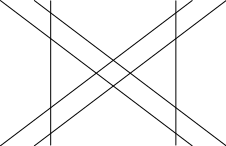
\includegraphics[width=\textwidth]{figures/intro_curves1.png}
    \caption{curves} \label{subfig:intro_unboundedFaces_a}
  \end{subfigure}%
  ~%
  \begin{subfigure}{.32\textwidth}
    
\includegraphics[width=\textwidth]{figures/intro_unboundedFaces_b.png}
    \caption{separate faces} \label{subfig:intro_unboundedFaces_b}
  \end{subfigure}%
  ~%
  \begin{subfigure}{.32\textwidth}
    
\includegraphics[width=\textwidth]{figures/intro_unboundedFaces_c.png}
    \caption{unified face} \label{subfig:intro_unboundedFaces_c}
  \end{subfigure}%
  \caption[xxx]
          {Two approaches for dealing with the exterior region, lying out of all faces.
          In this work we take the approach in figure~\ref{subfig:intro_unboundedFaces_c}.}
  \label{fig:subd_superface}
\end{figure}

%%%%%%%%%%%%%%%%%%%%%%%%%%%%%%%%%%%%%%%%%%%%%%%%%%%%%%%%%%%%%%%%%%%%%%%%%%%%%%%%
\subsection{Background}
\td{I still can't believe this problem has not been solved! :(}
%% Where the space $\mathcal{S}$ is two dimensional and the curve set $\mathcal{C}$ contains the level curves of only linear functions ($f(X)$).
%% \[ \mathcal{C} = \lbrace c_i \mid c_i: ax_1+bx_2+c=0, i \in I, \text{$I$: index set of $\mathcal{C}$} \rbrace \]
%% Consequently every face is a polygon bounded to line segments.


%%%%%%%%%%%%%%%%%%%%%%%%%%%%%%%%%%%%%%%%%%%%%%%%%%%%%%%%%%%%%%%%%%%%%%%%%%%%%%%%
\subsection{This work}

This work relies on the following assumptions:
\begin{description}
\item [Assumption 1] the space is a two dimensional plane.
\item [Assumption 2] if two curves were identical, their intersection would be the same curve which is beyond a finite set of points.
  In order to prevents the intersection procedure yielding a result other than a finite set of points, redundant curves are rejected so that;
  \[ \nexists c_i , c_j \in \mathcal{C}, \quad c_i = c_j \]
\item [Assumption 3] the set $\mathcal{C}$ contains levels curves resulted from either linear functions (straight lines as an example of an unbounded class) or conic sections (circles as an example of a bounded class).
\end{description}

\td{mention we are introducing circle curves
Then mention the challenges which the already existing methods would face in the presence of circles. }

\begin{figure}%[!ht]
  \centering
  \begin{subfigure}{.4\textwidth}
    \includegraphics[width=\textwidth]{figures/intro_curves2.png}
    \caption{curves} \label{subfig:intro_curves2}
  \end{subfigure}%
  \quad \quad \quad%
  \begin{subfigure}{.4\textwidth}
    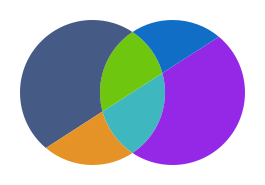
\includegraphics[width=\textwidth]{figures/intro_partitioning2.png}
    \caption{partitionaing} \label{subfig:intro_partitioning2}
  \end{subfigure}%
  \caption[xxx]
          {A planar subdivision, over a set of curves containing a straight line and two circles.
          Figure~\ref{subfig:intro_curves2} shows the set of curves, and the ``faces'' resulting from partitioning are color coded in figure~\ref{subfig:intro_partitioning2}.}
  \label{fig:intro_curvesPartitioning2}
\end{figure}

%%%%%%%%%%%%%%%%%%%%%%%%%%%%%%%%%%%%%%%%
\subsubsection{Challenges}
\td{briefly mention the challenges, such as membership function, holes, ...}

%% The first problem that rises from a non-convex region is, the expression of the region.
%% For instance the cross product won't work, therefore we need constraint-based description.

%% The circle in particular has a the circular behavior which means it is a closed (bounded) region.
%% Special case is where the circle resides inside a leaf, and with no intersection splits the leaf into sub-leaves.
